\subsection{時間分解能の電圧特性と研究目的}
先行研究\cite{Kita_Master}から、タイムウォーク$\sigma_{\rm{tw}}$、ランダウノイズ$\sigma_{\rm{L}}$の影響が少ない赤外線パルスレーザーを使った測定では、
時間分解能が以下の 図\ref{fg:Kita_JittervsVoltage} のようになる。横軸が印加電圧で縦軸が時間分解能である。
赤点が$50 \rm{\mu m}$厚のStrip型、緑点が$20 \rm{\mu m}$厚のStrip型、青点が$50 \rm{\mu m}$厚のPad型、橙色の点が$20 \rm{\mu m}$厚のPad型センサーである。
$50 \rm{\mu m}$厚のPad 型センサーは、電圧が180 V付近で時間分解能が最も良く、その前後の電圧で10 V程度の時間分解能の変化がほとんどない領域が存在する。
さらに電圧を印加すると、時間分解能が悪くなることがこの研究からわかっている。

そのため、本研究ではAC-LGAD 検出器の ASIC の開発に向けた基礎特性の理解として、最も良い時間分解能を実現する増幅率を決定することと、
今後のAC-LGAD検出器の時間分解能の向上をはかるために、特に増幅率が高い場合に時間分解能が悪化する原因について理解することを目的とする。

\begin{figure}[H]
    \centering
    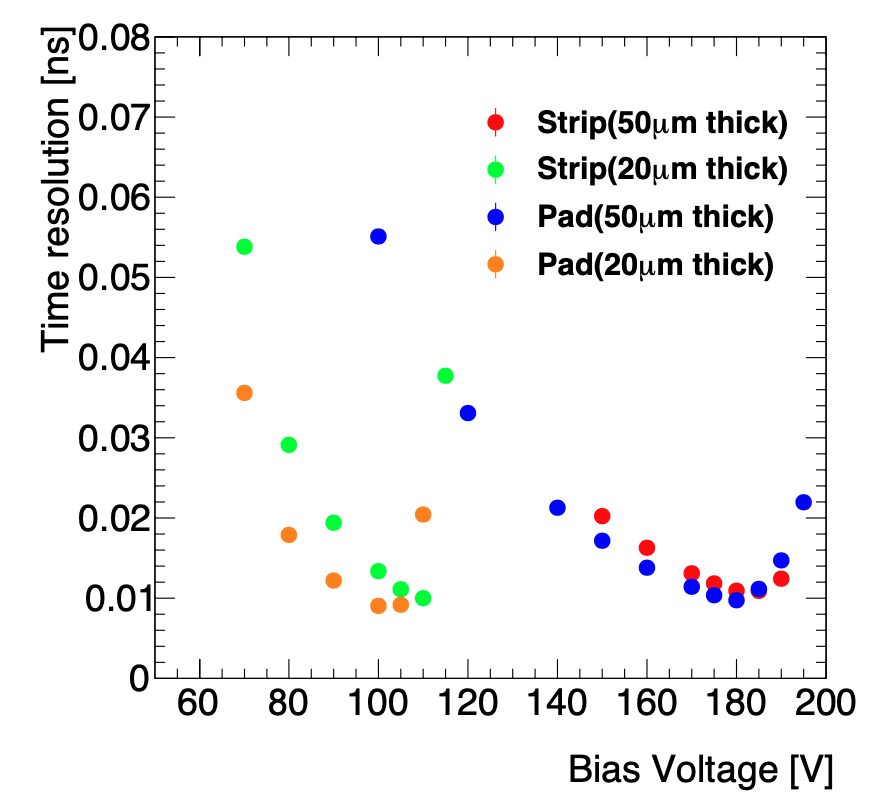
\includegraphics[width=8cm]{fig/ch1/Kita_JittervsVoltage.png}
    \caption[レーザーで測定した時間分解能(ジッター)\cite{Kita_Master}]{レーザーで測定した時間分解能(ジッター)\cite{Kita_Master}\\横軸が印加電圧で縦軸が時間分解能である。\\赤点が$50 \rm{\mu m}$厚のStrip型、緑点が$20 \rm{\mu m}$厚のStrip型、青点が$50 \rm{\mu m}$厚のPad型、橙色の点が$20 \rm{\mu m}$厚のPad型センサーである。
    $50 \rm{\mu m}$厚のPad 型センサーを示している。}
    \label{fg:Kita_JittervsVoltage}
\end{figure}
